\noindent

\includegraphics[height=1.25cm]{images/pictograms/under_construction}

\includegraphics[height=1.25cm]{images/pictograms/tools}

\includegraphics[height=1.25cm]{images/pictograms/paraview}

%%%%%%%%%%%%%%%%%%%%%%%%%%%%%%%%%%%%%%%%%%%%%%%%%%%%%%%%%%%%%%%%%%%%%%%%%%%%%%%%%%%%%%%%%%%%%%%%%%%

\begin{flushright} {\tiny {\color{gray} python\_codes/fieldstone\_159/text.tex}} \end{flushright}

%\lstinputlisting[language=bash,basicstyle=\small]{python_codes/template_keywords.key}

\par\noindent\rule{\textwidth}{0.4pt}

\begin{center}
\inpython
{\small Code: \url{https://github.com/cedrict/fieldstone/tree/master/python_codes/fieldstone_159}}
\end{center}

\par\noindent\rule{\textwidth}{0.4pt}

%%%%%%%%%%%%%%%%%%%%%%%%%%%%%%%%%%%%%%%%%%%%%%%%%%%%%%%%%%%%%%%%%%%%%%%%%%%%%%%%%%%%%%%%%%%%%%%%%%%

The goal of this \stone is to explore, check and plot the yield envelopes of 
the main plastic yield criteria.
We will here focus on:
\begin{itemize} 
\item von Mises
\item Tresca
\item Mohr-Coulomb
\item Drucker-Prager (all three variants)
\end{itemize} 
The four models are parameterized by a cohesion $c$ and an angle of friction $\phi$. 

The code works as follows: We will explore a stress 
space $\{\sigma_1,\sigma_2,\sigma_3\}\in[-\sigma_{max},\sigma_{max}]^3$.
For each point inside this domain, we compute the 1st, 2nd and 3rd moment invariants, i.e.
\[
\III_1({\bm \sigma}), 
\qquad \III_2({\bm \tau}), 
\qquad \III_3({\bm \tau}), 
\qquad \uptheta_{\rm L}\in[-\pi/6,\pi/6]
\] 
At each point we will then evaluate the yield function $\FFF$. 
If {\python make\_vtu} is True, a (very large) vtu file will be produced (in this 
case nnx should not exceed 200).
The code exports the point that fulfill $\FFF=0$ within 10~\si{\kilo\pascal}. 
which allows to trace the yield envelopes.
The same can be achieved by opening the vtu file and looking at zero isocontours of each $\FFF$ field.

We set $c=20~\si{\mega\pascal}$ and $\phi=20\degree$. After trial an error, we set $\sigma_{max}=60MPa$.

The first invariant of the stress tensor is given by 
\[
\III_1({\bm\sigma})=\sigma_{xx}+\sigma_{yy}+\sigma_{zz} = \sigma_1+\sigma_2+\sigma_3
\]
which translates into
\begin{lstlisting}
I1sig=x+y+z
\end{lstlisting}
The second invariant of the deviatoric stress tensor is given by 
\[
\III_2({\bm \tau})  
=\frac{1}{6}\left[(\sigma_{xx}-\sigma_{yy})^2 + (\sigma_{yy}-\sigma_{zz})^2 + (\sigma_{xx}-\sigma_{zz})^2 \right]  
+ \sigma_{xy}^2 + \sigma_{xz}^2 + \sigma_{yz}^2 
\]
In the case of a diagonal stress tensor then
\[
\III_2({\bm \tau})  
=\frac{1}{6}\left[(\sigma_{1}-\sigma_{2})^2 + (\sigma_{2}-\sigma_{3})^2 + (\sigma_{1}-\sigma_{3})^2 \right]  
\]
which translates into
\begin{lstlisting}
I2tau=((x-y)**2+(x-z)**2+(y-z)**2)/6.
sqrtI2tau=np.sqrt(I2tau)
\end{lstlisting}

The third invariant is given by
\[
\III_3(\bm \tau)
= \frac{1}{81}
\left[
(2\sigma_1-\sigma_2-\sigma_3)^3+
(2\sigma_2-\sigma_1-\sigma_3)^3+
(2\sigma_3-\sigma_1-\sigma_2)^3
\right] 
\]
which translates into
\begin{lstlisting}
I3tau=((2*x-y-z)**3+(2*y-x-z)**3+(2*z-x-y)**3)/81.
\end{lstlisting}

Finally the Lode angle is given by
\[
\uptheta_{\rm L} = 
=\frac{1}{3} \sin^{-1} 
\left( -\frac{3\sqrt{3}}{2} \frac{{\III}_3({\bm \tau})}{{\III}_2({\bm \tau})^{3/2}} \right)
\]
and is implemented as follows:
\begin{lstlisting}
theta=-3*np.sqrt(3)/2*I3tau/sqrtI2tau**3
theta=min(theta,0.99999999)
theta=max(-0.99999999,theta)
theta=np.arcsin(theta)/3.
\end{lstlisting}

When ran at high resolution, one can extract the following plots:
\begin{center}
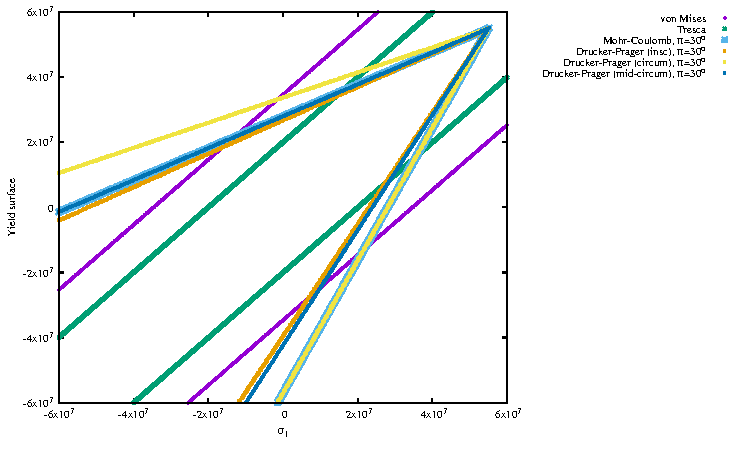
\includegraphics[width=12cm]{python_codes/fieldstone_159/images/surfaces_xy.pdf}
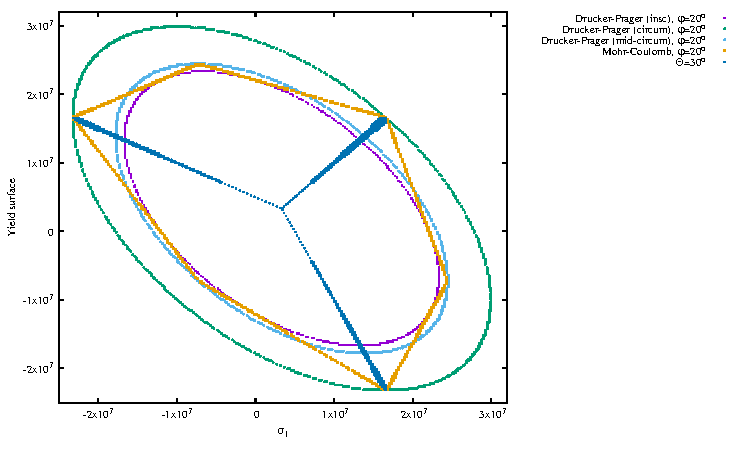
\includegraphics[width=12cm]{python_codes/fieldstone_159/images/surfaces_plane.pdf}
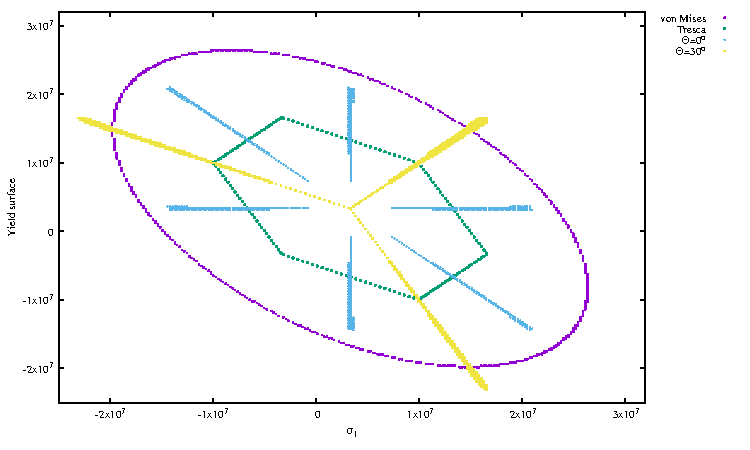
\includegraphics[width=12cm]{python_codes/fieldstone_159/images/surfaces_plane2.pdf}\\
{\captionfont Obtained with nnx=512}.
\end{center}

Using paraview on the {solution.vtu} file, and plotting zero-isocontours of each yield function:
\begin{center}
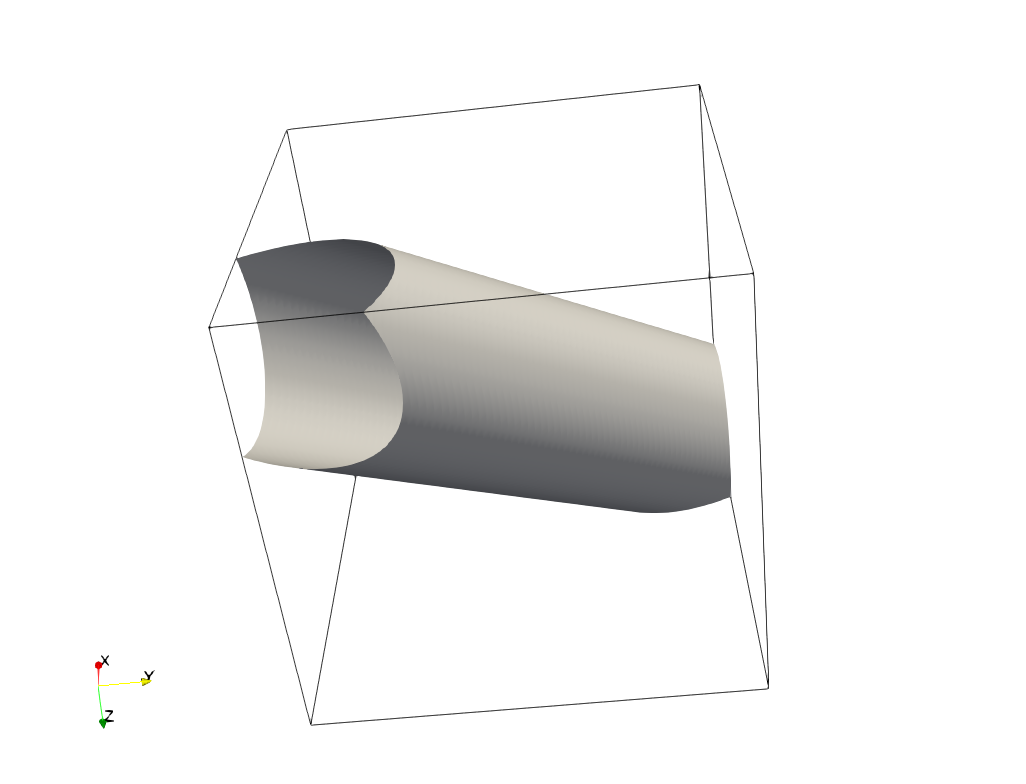
\includegraphics[width=6cm]{python_codes/fieldstone_159/images/VM}
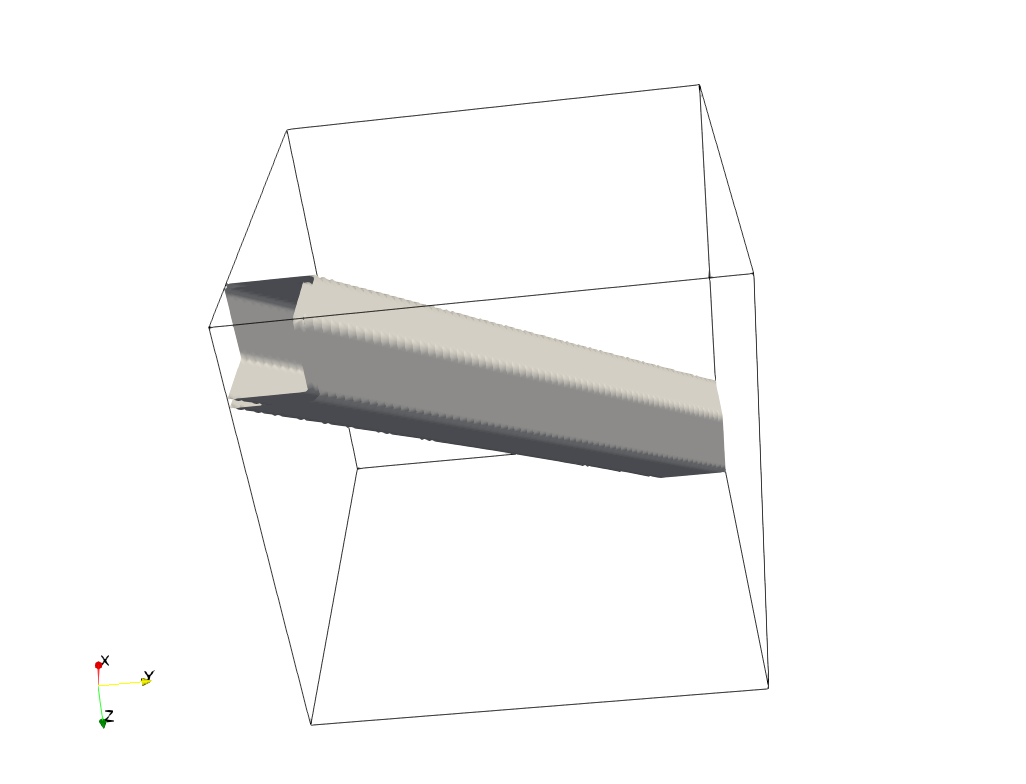
\includegraphics[width=6cm]{python_codes/fieldstone_159/images/TR}\\
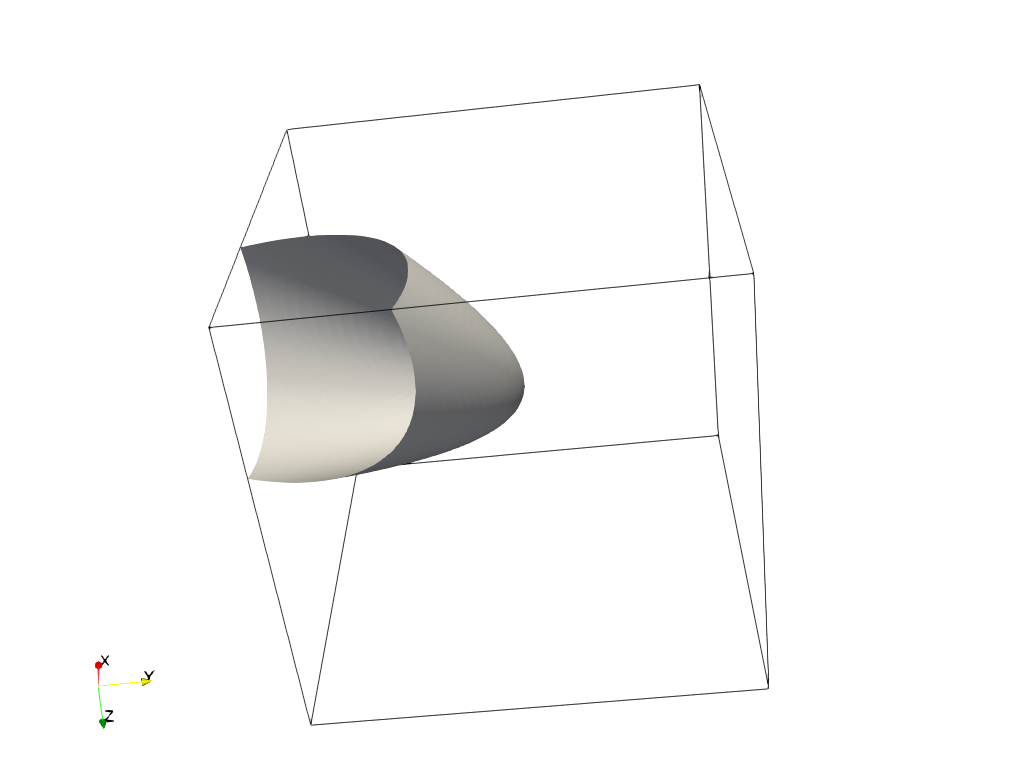
\includegraphics[width=6cm]{python_codes/fieldstone_159/images/GM}
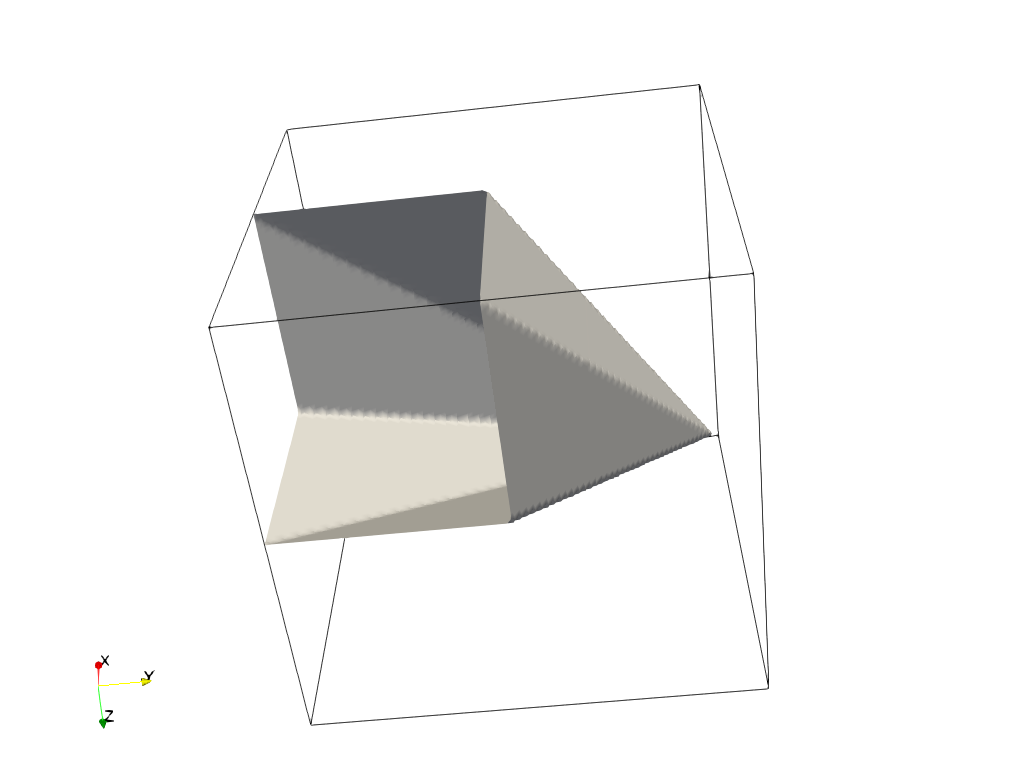
\includegraphics[width=6cm]{python_codes/fieldstone_159/images/MC}\\
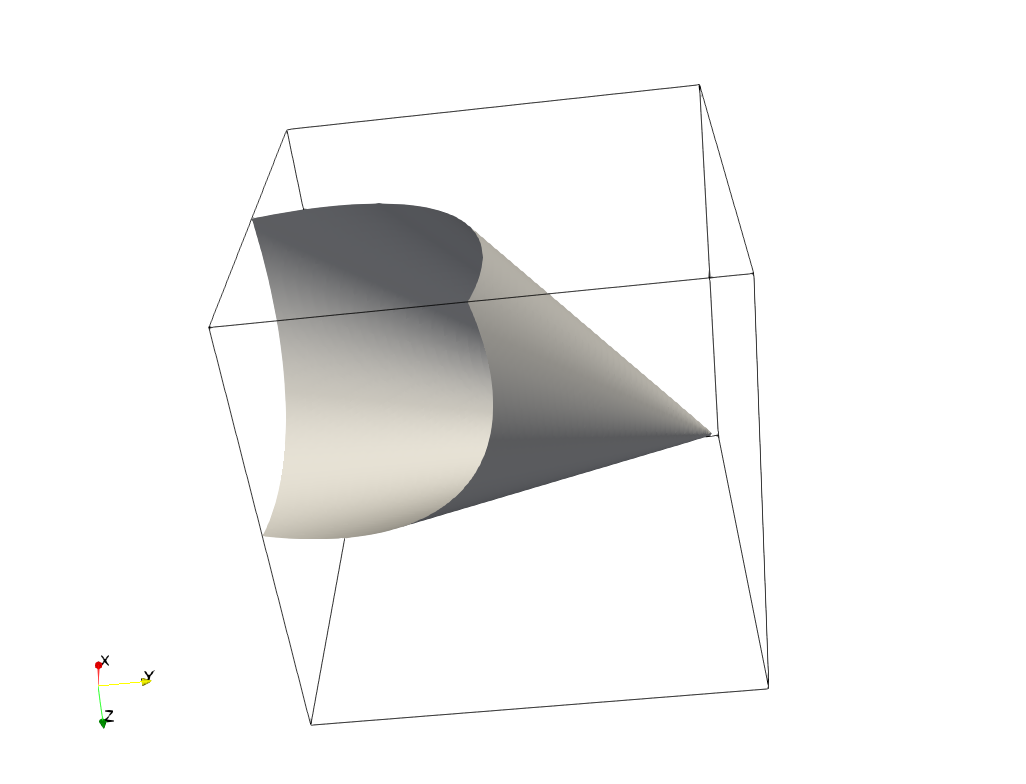
\includegraphics[width=5.7cm]{python_codes/fieldstone_159/images/DPi}
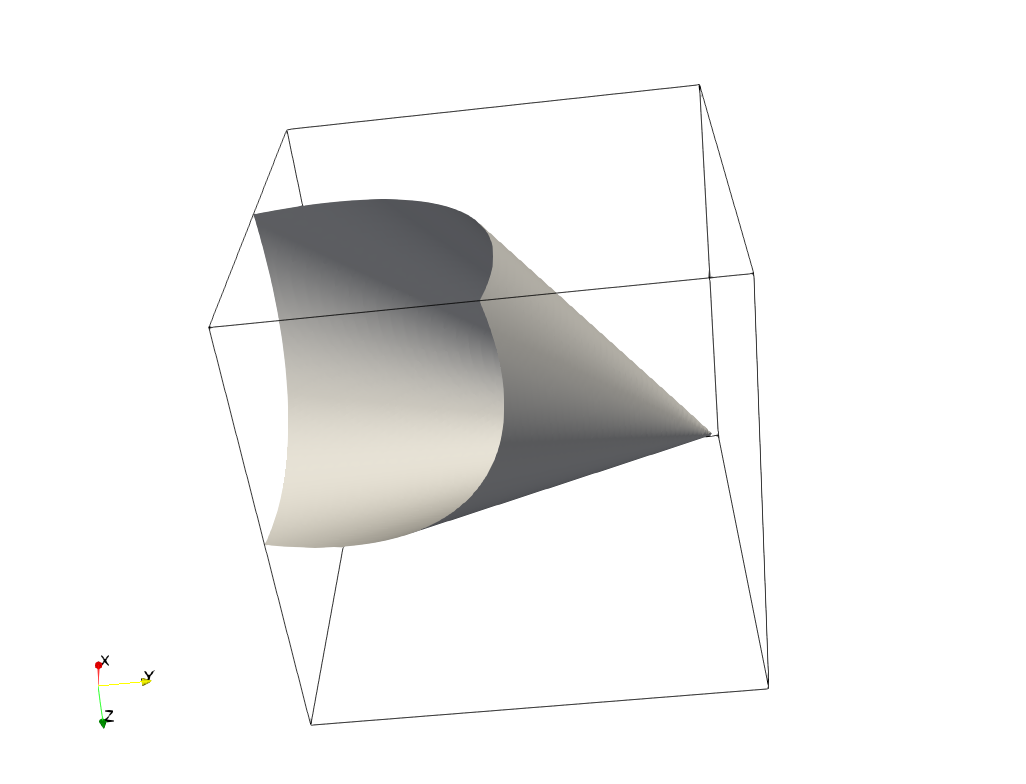
\includegraphics[width=5.7cm]{python_codes/fieldstone_159/images/DPm}
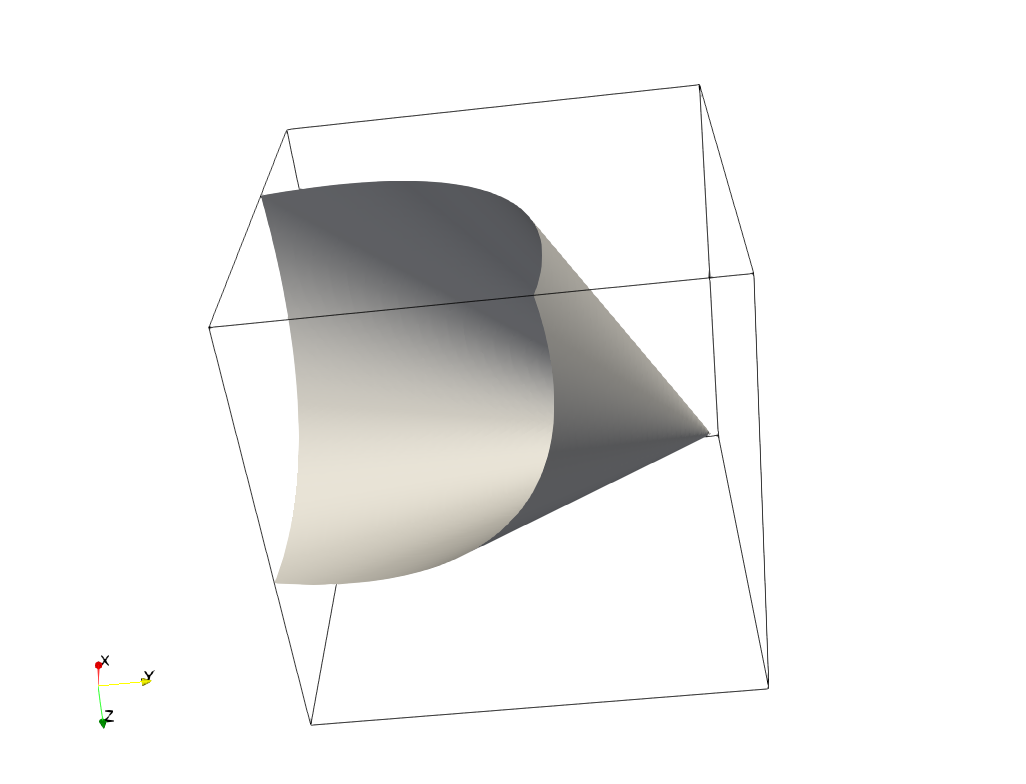
\includegraphics[width=5.7cm]{python_codes/fieldstone_159/images/DPc}
{\captionfont Obtained with nnx=80}.
\end{center}

WHy is tresca so far from vM ?

not sure how to choose the parameter for GM, so after trial and error I took c/20.


